\documentclass{beamer}

\usepackage{subfigure}
\usepackage{graphicx}
\usepackage{sidecap}
\usepackage{caption}
%\usepackage{subcaption}
\captionsetup{compatibility=false}
\usepackage{appendixnumberbeamer}
\usepackage{amsmath}
% --
\usepackage{multirow}
\usepackage{xcolor}
\usepackage{setspace}
\usepackage{hyperref}
\usepackage{anyfontsize}

\beamertemplatenavigationsymbolsempty
\setbeamertemplate{footline}

\newenvironment{itemise} {\begin{itemize} \setlength{\itemsep}{0.2cm}} {\end{itemize}}
\usepackage[labelformat=empty]{caption}
\setbeamertemplate{sections/subsections in toc}[square]

%% COLORS
\definecolor{Gray}{gray}{0.9}
\definecolor{dblue}{rgb}{0.132,0.1,0.27}
\definecolor{mint}{cmyk}{1.0, 0.2, 0.6, 0.05}
\definecolor{ant}{cmyk}{0.5, 0.1, 0.0, 0.45}
\definecolor{lgray}{cmyk}{0.12, 0.0, 0.0, 0.17}
\definecolor{lred}{cmyk}{0.0, 0.9, 0.7, 0.0}


\usepackage{etoolbox}% http://ctan.org/pkg/etoolbox 
\usepackage{booktabs}

\newenvironment{literatur}{%
  \parskip2pt \parindent0pt \raggedright
  \def\lititem{\hangindent=0.5cm \hangafter1}}{%
  \par\ignorespaces}

\newcommand{\tb}[1]{{\color{blue}{\textbf{#1}}}}
\newcommand{\tm}[1]{{\color{mint}{\textbf{#1}}}}
\newcommand{\tr}[1]{{\color{red}{\textbf{#1}}}}
\newcommand{\tbs}[1]{{\color{blue}{#1}}}
\newcommand{\trs}[1]{{\color{red}{#1}}}
\newcommand{\tms}[1]{{\color{mint}{#1}}}
\newcommand{\tps}[1]{{\color{purple}{#1}}}
% Ilya: packages

\usepackage{tikz}
\usepackage{lmodern}
\usepackage{enumitem}

% Ilya: my commands

\newenvironment{mytemize}
{\vfill\itemize[nolistsep,itemsep=\fill,label=\color{blue}{$\triangleright$}]}
  {\enditemize}

\newenvironment{mynumerate}
{\vfill\enumerate[nolistsep,itemsep=\fill,label=\arabic*.]}
  {\endenumerate}

\newcommand{\hitem}[1]{
  {\color{blue}{$\triangleright$}} 
  {#1} 
  {\hfill}
}

\setlist[itemize]{label= \color{blue}{$\triangleright$}}
\setlist[enumerate]{label = \arabic*.}

\newcommand{\rarr}{$\Rightarrow$\ }


\AtBeginSection{%
\begin{frame}
    \tableofcontents[currentsection, subsectionstyle=show/show/hide]
\end{frame}
}
\AtBeginSubsection{%
\begin{frame}
    \tableofcontents[currentsubsection]
\end{frame}
}

%\href{<Ziel>}{<Eingefasster Text>} 

%\logo{\includegraphics[height=0.7cm]{BdFlogo.eps}\hspace{300pt}\vspace{-5pt}}
%\logo{\includegraphics[height=0.8cm]{BdFlogo.eps}}
%\logo{\pgfputat{\pgfxy(-6.2,-0.5)}{\pgfbox[center,base]{\includegraphics[height=0.8cm]{BdFlogo.eps}}}}

%------------------------------------------------------------------------------------
% TITLE
%------------------------------------------------------------------------------------
\title[PSME]{Macroeconomics\\ Lecture 6 -- Labor \& Intro to Real Business Cycles }
\author[I. Eryzhenskiy]{Ilya Eryzhenskiy}
\institute[BdF]{PSME Panth\'{e}on-Sorbonne Master in Economics}
\date[PSME macro]{Fall 2023}

\begin{document}

\begin{frame}
   \maketitle 
\end{frame}

\begin{frame}{Overview}
    \tableofcontents
\end{frame}

\section{Labor supply: consumption-leisure choice}

\subsection{One-period version}
\begin{frame}{Labor: extensive vs. intensive margin}
    \begin{mytemize}
        \item \tb{Extensive margin}: do I work at all?
            \begin{mytemize}
                \item Not always a choice: voluntary vs. involuntary unemployment
                \item \tr{No theory for this in this course}
            \end{mytemize}
        \item \tb{Intensive margin}: how much do I work?
        \begin{mytemize}
                \item An easier question for neoclassical economics
                \item \tb{Leisure} modelled as a \textbf{good} \\ \rarr Labor time $=$ Total time endowment $-$ Leisure time
            \end{mytemize}
    \end{mytemize}
\end{frame}

\begin{frame}{Consumption-leisure choice}
  Consider a household with total endowment of time equal to 1 (normalization) \\ $N$ is \textbf{share} of time devoted to work, $L=1-N$ is \textbf{share} of time devoted to leisure. \vfill 
  Household cares for consumption $C$ and leisure time $1-N$:
  \begin{equation*}
	U(\underset{+}{C}, \underset{+}{L}) =  U(\underset{+}{C}, \underset{+}{1-N}) \quad \text{or, equivalently,} \quad \tilde U(\underset{+}{C}, \underset{-}{N})
  \end{equation*} 
%  Examples of utility function:  \\
%  $\ln C + \alpha \ln(1-N)$ \\ $\ln C - \alpha/(1+\chi) L^{1+\chi}$ -- in this case, $\chi$ is the inverse of Frisch  elasticity of labor supply -- labor supply under fixed marginal utility of income.
  Denote $W$ nominal wage, $w = W/P$ real wage. \\ Budget constraint:
  \begin{align*}
	P \cdot C \leq  W \cdot N &\Leftrightarrow C \leq w N \\
		&\Leftrightarrow C + w (1-N) \leq w \quad \text{(consumption vs. leisure)}
  \end{align*} 
  Real wage acts as \textbf{opportunity cost}, or price, of leisure
\end{frame}

\begin{frame}{Consumption-leisure choice: analytical solution}
\vspace{-3.5cm}
\begin{align*}
\max_{C\geq 0, N \in (0,1)} &U(C,1-N) \\ \text{s.t.} \quad &C + w (1-N) = w 
\end{align*}
When solving, note that $U$ here is really a function of $L$, not $N$, so $$\frac{\partial U(C, 1-N)}{\partial N} = - U'_L(C, 1-N)$$ 
\end{frame}

\begin{frame}{Consumption-leisure choice: graphical solution}
    
\end{frame}

\begin{frame}{Consumption-leisure choice: comparative statics}
\vspace{-4.5cm}
   With an increase of $w$, leisure can either increase or decrease. Typically, substitution effect dominates \rarr leisure decreases \rarr \textbf{more labor supplied when wage is higher} 
\end{frame}

\subsection{Multi-period version}
\begin{frame}{Consumption-leisure with many periods}
\begin{align*}
\max_{\{C_t\}\geq 0, \{N_t\} \in (0,1)} &\sum_{t=0}^\infty \beta^t u(C_t,1-N_t) \\ \text{s.t.} \quad &C_t + S_t = w_t N_t + (1+r_{t-1}) S_{t-1} 
\end{align*}
Now the \tb{instanteneous utility function} of every period has two arguments \vfill
The consumption-leisure choice is \textbf{static}: it only involves variables of one period \rarr same consumption-leisure optimality condition as before:
$$\frac{u'_L(C_t, 1-N_t)}{u'_C(C_t, 1-N_t)} = w_t$$

\end{frame}

%\begin{frame}{Consumption and leisure with 2 periods: Lucas-Rapping effect}
%  Now consider a 2-period problem with both consumption and leisure. We will assume a specific form of utility function to simplify analysis:
%  \begin{align*}
%	\max_{C_1, C_2, L_1, L_2}  \{\ln C_1 - \gamma \sigma/(1&+\sigma) L_1^{(1+\sigma)/\sigma}  \\
%	&+ \beta(\ln C_2 - \gamma \sigma/(1+\sigma) L_2^{(1+\sigma)/\sigma})\} \\
%	\text{s.t.} \quad C_1 + C_2/(1+r) &= w_1 L_1 + w_2 L_2 / (1+r)
%  \end{align*}
%  
%\end{frame}
%\begin{frame}{Consumption and leisure with 2 periods: solution}
%\end{frame}
%
\begin{frame}{Consumption-leisure with many periods: Lucas-Rapping effect}
  Consider the following comparative statics with many periods: a one-period increase in wage in $t$. We will assume that the substitution effect dominates: $N_t$ depends positively on $w_t$. How is labor supply affected in $t+1, t+2 ...$?
  \begin{mytemize}
  \item With higher wage in $t$, hours worked are above average, additional savings $S_t$ are made
  \item From $t+1$ on, wage back to normal. A rational consumer now spends savings from previous period $S_t$ and works \textbf{below average} hours
  \item This continues until the extra savings made in $t$ are consumed
  \end{mytemize}
  \vfill
  The below-average work effort  (\tb{Lucas-Rapping effect}) comes from leisure being \textbf{normal good}: with more wealth, you want both \textbf{more consumption} and \textbf{more leisure}. 
\end{frame}
%---FRAME------------------------------------------------------------------------------

\section{Explaining business cycles with a dynamic model}

\subsection{Lucas critique}
\begin{frame}{Why micro in macro? Some history}

\begin{mytemize}
\item Empirical macro used to be done as estimation of \textbf{big} systems of equations with OLS-like methods
\item[\rarr] IS-LM (IS-TR), Mundell-Flemming (IS-TR-IFM), AD-AS models were brought to data like:
\end{mytemize}
\begin{figure}[h!]
%\caption{Figure. Net}
	\subfigure{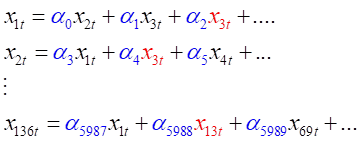
\includegraphics[trim=0 0 0 0,clip,width=0.5\textwidth]{FIGURES/9_LCritiqueMatrix}
	}      
	%} 		
%	\label{fig:GPD} 
	%[trim=left bottom right top
\end{figure}

\begin{mytemize}
\item Robert Lucas' idea in 1976 (\tb{Lucas critique}): The parameters (e.g. marginal propensity to consume) are \textbf{endogenous} with respect to government policy
\end{mytemize}
\end{frame}
\begin{frame}{Lucas critique: examples}
  Consider households' reaction to a change in taxes, e.g. a new carbon tax:
  \begin{mytemize}
  \item Is it temporary or permanent? Very different consumption responses (mpc's)
  \item What are implications for the government budget? Households realize that the whole macro equilibrium may change with big changes in tax, e.g. a recession might follow \rarr more savings needed 
  \item Labor supply interacts with consumption demand, as seen above
  \end{mytemize}
\end{frame}

\begin{frame}{Lucas critique: response}
  
  Two essential elements of modern models address Lucas' critique:
  \begin{mynumerate}
	\item All agents optimize some objective function. Utility for households, profit for firms.
	\item \tb{Rational expectations}: agents know the structure of the economy (the model), errors are possible, but not \textbf{systematic} 
  \end{mynumerate}
  \vfill 
  This is how macroeconomics became micro-founded and the \tb{Real Business Cycles (RBC)} model was created \vfill
  Later on, the model was extended to include sticky price components -- the \tb{New Keynesian model} was created
\end{frame}
%---FRAME------------------------------------------------------------------------------
%\section{Overview}

\subsection{RBC framework}

\begin{frame}{RBC model: structure}
    \begin{mytemize}
        \item \underline{Households} maximize expected utility by:
        \begin{mytemize}
            \item supplying labor \rarr earning wage
            \item consuming, saving by investing in (1) bonds (2) firm capital \rarr earning \textbf{interest on bonds} and \textbf{return on capital}
        \end{mytemize}
        \item  \underline{Firms} maximize expected profits by: 
        \begin{mytemize}
            \item producing goods with labor and capital...
            \item ...subject to \tb{productivity shocks}
        \end{mytemize}
        \item Flexible prices \rarr goods, labor, capital and bond markets in equilibrium
        
    \end{mytemize}
\end{frame}

\begin{frame}{Productivity shocks: a key element}
    Production with labor $N_t$ and physical capital $K_t$ is modelled as:
    $$Y_t = A_t F(K_t, N_t)$$
    $A_t$ is \tb{total factor productivity (TFP)} and it is a \textbf{random variable} in the model. It is usually assumed to follow an autoregressive process in logs, so that it has some \tb{persistence}:
    $$\ln A_t = \rho \ln A_{t-1} + \varepsilon_t$$
    \tr{This is the only source of business cycles in the classical RBC model.} One either simulates a one-period shock in $t=0$ ($\varepsilon_0 > 0, \varepsilon_t = 0$ for $t>0$) and studies \tb{impulse response} or does a \tb{stochastic simulation} with shocks happening every period and $\quad \varepsilon_t \sim \mathcal N (0, \sigma^2_\varepsilon)$ \vfill
    Possible to introduce other shocks than TFP, but it is TFP shocks that make model variables behave most like the empirical macro time series
\end{frame}
\begin{frame}{Model and data: stationarity}
   RBC models produce \tb{stationary} paths for macro variables by construction \vfill
   Stationary $\approx$ mean reverting: variables tend to converge to their mean, which is also \tb{steady state} of the model \vfill

   This is not usually the case for macro time series: they are non-stationary \vfill
   Two problems created by non-stationarity:
   \begin{enumerate}
       \item Hard to compare to model output
       \item \tb{Spurious correlations}: time series seem related even if they aren't 
   \end{enumerate}
   \vfill
   \rarr Need to transform macro series to have them in stationary form

    
\end{frame}

\subsection{Macro data processing}
\begin{frame}{Macro data processing}
    
 Steps to transform macro data to make it comparable to model output:
    \begin{mynumerate}
        \item Remove \tb{seasonality} from data (done by macro data providers in most cases; but you will also learn to de-season in TD)
        \item Obtain percentage deviations from \tb{trend} by: 
        \begin{mynumerate}
            \item taking a logarithm of your variable \trs{(not needed for interest rates -- they are already percentages)}
            \item subtracting the the log of trend value: $\ln(x_t) - \ln(x^{trend}_t) = \underbrace{\ln\left(\frac{x_t}{x^{trend}_t}\right) = \ln\left(1+\frac{x_t - x^{trend}_t}{x^{trend}_t}\right)}_{\tms{\text{verify this step}}}$
            and $\ln\left(1+\frac{x_t - x^{trend}_t}{x^{trend}_t}\right) \approx \frac{x_t - x^{trend}_t}{x^{trend}_t}$  using $\ln(1+x) \underset{x \to 0}{\to} x$. \\
    \end{mynumerate}
    We get \tbs{$\ln(x_t) - \ln(x^{trend}_t) \approx \frac{x_t - x^{trend}_t}{x^{trend}_t}$}: deviation of variable from trend in percent of the trend value of the period $\rightarrow$ our preferred measure of business cycle
    \end{mynumerate}
\end{frame}

\begin{frame}{What is the trend?}
Reminder: two different ideas of \tb{trend GDP} in course: 
\begin{mynumerate}
    \item Trend GDP is GDP in flexible-price equilibrium -- was contrasted with Keynesian equilibria in IS-TR, medium-term AS-AD
    \item Trend GDP is literally the trend -- GDP time series that has been smoothed using statistical procedures
\end{mynumerate} \vfill
In empirical business cycle research, the smoothing idea is used \\ \vfill
Defined this way, deviations from trend (i.e. business cycles) can exist under flexible prices, too

\end{frame}

\begin{frame}{Trend as smoothing of series: two procedures}
Two options for smoothing the series $\{x_t\}_{t=1}^T$ -- e.g. GDP:
\begin{mynumerate}
    \item Run OLS on linear time trend (possibly \tps{quadratic trend}, too); use fitted values: 
    $$(\hat \beta_0, \hat \beta_1, \tps{\hat \beta_2}) = \text{argmin} \sum_{t=1}^T \left(x_t -  \beta_0 - \beta_1 \cdot t \tps{-\beta_2 \cdot t^2}\right)^2$$
    Then, $x^{trend}_t = \hat x_t = \hat \beta_0 + \hat \beta_1 \cdot t \tps{+ \hat \beta_2 t^2}$
    \item Run HP filter:
    \begin{align*}
        \{x^{trend}_t\}_{t=1}^T = \text{argmin} \left[\sum_{t=1}^{T}\right. &(x_t - x^{trend}_t)^2 \\ + \lambda \sum_{t=2}^{T-1}( (&x^{trend}_{t+1} - x^{trend}_t) \left.- (x^{trend}_{t} - x^{trend}_{t-1}))^2\right]
    \end{align*}
Where $\lambda$ is a parameter that regulates smoothness of the trend. With $\lambda \to \infty$, trend linear. 
\end{mynumerate}
\end{frame}


\begin{frame}{Checking stationarity}
    Once the data is transformed, we check whether it is \tb{stationary} in two ways:
    \begin{enumerate}
        \item Visually -- does the series seem to always return to the mean?
        \item Statistical tests of Dickey-Fuller (DF) type  
    \end{enumerate}
    \vfill
    Idea of DF test: if process is AR(1): $x_t = \rho x_{t-1}+\varepsilon_t$ with $\rho \leq 1$, then it is non-stationary (random walk) if $\rho =1$. \vfill
    Instead of testing $\rho = 1$ directly, subtract $x_{t-1}$ from both sides: 
    $$\underbrace{x_t - x_{t-1}}_{\Delta x_t} = \underbrace{(\rho-1)}_{\trs{\delta}} x_{t-1} + \varepsilon_t$$
    and test significance of \trs{$\delta$} (not t-stat, but a special DF-stat used). \vfill

    In practice, you will use Augmented Dickey-Fuller (ADF) that also includes several lags of $\Delta x_t$ on the right hand side, and can allow for a constant term and/or linear time trend (not needed if you have de-trended first). 
\end{frame}

\subsection{Basic RBC model vs. data}
\begin{frame}{RBC models vs. data}
    RBC models take \textbf{long-run} empirical facts about market economies as \textbf{assumptions} and then seek to reproduce \textbf{short-run} or \textbf{medium-run} behaviour of economies \vfill

    Long-run ``stylized facts'' (Kaldor, Kuznets):
    \begin{mynumerate}
        \item Stable relationship between investment and GDP
        \item Stable share of labor income in GDP (less stable recently -- see work of Piketty)
        \item Stable hours per worker
    \end{mynumerate} \vfill
    Short-run \tb{second-order moments}, i.e. variances, correlations:
    \begin{mynumerate}
        \item Variance of consumption smaller than variance of GDP, smaller than variance of investment
        \item All main macro aggregates \tb{procyclical}: positive correlation to GDP cycle 
    \end{mynumerate}
\end{frame}
\begin{frame}{U.S. economy: Business Cycle moments}
 \begin{table}
    \centering    
    \begin{tabular}{|c|c|c|c|c|}

    \hline
         Variable $x_t$&  \multicolumn{4}{|c|}{Moments} \\
         \cline{2-5}
         &  $\sigma_{x}$&  $\frac{\sigma_x}{\sigma_{GDP}}$ &  corr$(x_t,x_{t-1})$&  corr$(x_t,GDP_t)$ \\
         \hline
         GDP&  1.81&  1.00&  0.84&  1.00\\
         Consumption&  1.35&  0.74&  0.80&  0.88\\
         Investment &  5.30&  2.93&  0.87&  0.80\\
         Work hours &  1.79&  0.99&  0.88&  0.88\\
         Real wage &  0.68&  0.38&  0.66&  0.12\\
         Real interest &  0.30&  0.16&  0.60&  -0.35\\
         Total factor productivity &  0.98&  0.54&  0.74&  0.78\\
         \hline
    \end{tabular}
    \vfill
    \centering{All variables except $r$ in logs and with HP filter. Total factor productivity (TFP) computed as a Solow residual: $\ln(TFP_t) = \ln Y_t - \hat \alpha \ln K_t - (1-\hat \alpha) \ln N_t $} 
    \label{tab:my_label}
\end{table}
   
\end{frame}


\begin{frame}{A basic RBC calibrated to match U.S.}
Moments of time series obtained from stochastic simulation (TFP shocks happenning every period) 
 \begin{table}
    \centering    
    \begin{tabular}{|c|c|c|c|c|}

    \hline
         Variable ($x_t$)&  \multicolumn{4}{|c|}{Moments} \\
         \cline{2-5}
         &  $\sigma_{x}$&  $\frac{\sigma_x}{\sigma_Y}$ &  corr$(x_t,x_{t-1})$&  corr$(x_t,Y_t)$ \\
         \hline
         Y &  1.39&  1.00&  0.72&  1.00\\
         C&  0.61&  \tbs{0.44}&  0.79&  0.94\\
         I&  4.09&  \tbs{2.95}&  0.71&  0.99\\
         N&  0.67&  \trs{0.48}&  0.71&  0.97\\
         w&  0.75&  0.54&  0.76&  \trs{0.98}\\
         r&  0.05&  \tbs{0.04}&  0.71&  \trs{0.95}\\
         A (TFP) &  0.94&  0.68&  0.72&  1.00\\
         \hline
    \end{tabular}
    \caption{}
    \label{tab:my_label}
   Key empirical facts matched well: \tbs{$\sigma_C < \sigma_Y, \sigma_I > \sigma_Y$}, high autocorrelation and procyclicality of all variables except $r$. 
\end{table}
   
\end{frame}

%
%\begin{frame}{Open Economy Business Cycle: Canada}
%  Canada -- developed economy, but 2.1 \% of world GDP \rarr ``small'' (compare to China -- 18.4\%; USA -- 24\% -- large open economies). 
%  \vfill
% Historical business-cycle patterns: 1946-1985.
%  \vfill
%\centerline{
%\begin{tabular}{|c|c|c|c|}
%\hline
%Variable ($x_t$)&\multicolumn{3}{|c|}{Moments}\\
%\cline{2-4}
%&$\sigma_{x_t}$
%&corr$(x_t,x_{t-1})$
%&corr$(x_t,Y_t)$
%\\
%\hline
%GDP           &  2.8&  0.61&      1\\
%Consumption           &  2.5&   0.7&   0.59\\
%Investment           &  9.8&  0.31&   0.64\\
%Work hours           &    2&  0.54&    0.8\\
%$\tbs{\frac{\text{Trade balance}}{\text{GDP}}}$&  \tbs{1.9}&  \tbs{0.66}&  \tbs{-0.13}\\
%\hline
%\end{tabular}}
%
%\centering{Source: Mendoza AER, 1991. Annual data. Log-quadratically detrended.}

\end{frame}

\end{document}